\section{Durchführung}
\label{sec:Durchführung}
In diesem Versuch wird versucht die Elementatladung $\epsilon_0$, sowie die Advogradokonstante $\symup{N}_{\text{A}}$ und die Faraday-Konstante zu bestimmen. Dies soll über die 
\textit{Milikan Öltröpfchenmethode} geschehen. Dazu wird zunächst eine Messapparatur gemäß \autoref{fig:aufbau} verwendet. Die einzelnen Bauelemente werden in der Abbildung 
mit der jeweiligen Nummer bezeichnet. Abstrakt beschrieben benötigt man für diesen Versuch lediglich einen Plattenkondensator, in welchem ein Magnetfeld erzeugt wird. Dieses 
muss parallel zu Richtung der Gravitationskraft gerichtet sein. Die Kammer soll in dieser Durchführung mit Luft gefüllt sein. Oben im Plattenkondensator findet sich eine 
Öffnung durch welche Öl in die Apparatur eingeführt werden kann. An der Seite des Plattenkondensators wird eine Halogenlampe verwendet, damit die Öltröpfchen sichtbarer werden.
Unterhalb des Plattenkondensator befindet sich ein radioaktives $\alpha$-Präparat. Dieses kann über einen Hebel das Öl bestrahlen, um so die Ladung dieser Öltröpfchen zu
verändern. Die \textit{"Kammer"} des Plattenkondensators kann über ein anliegendes Mikroskop beobachtet werden. Durch das Teleskop sind die Öltröpfchen mit einem Gitter im 
Hintergrund zu sehen. Der Abstand zweier \textit{dicker} Linien beträgt $\qty{0.5}{\milli\metre}$. Der Abstand zweier \textit{dünner} Linien zueinander beträgt 
$\qty{0.1}{\milli\metre}$. Damit das Öl in kleine Tröpfen aufgespalt wird, soll ein \textit{Zerstäuber} verwendet werden.

\begin{figure}
    \centering
    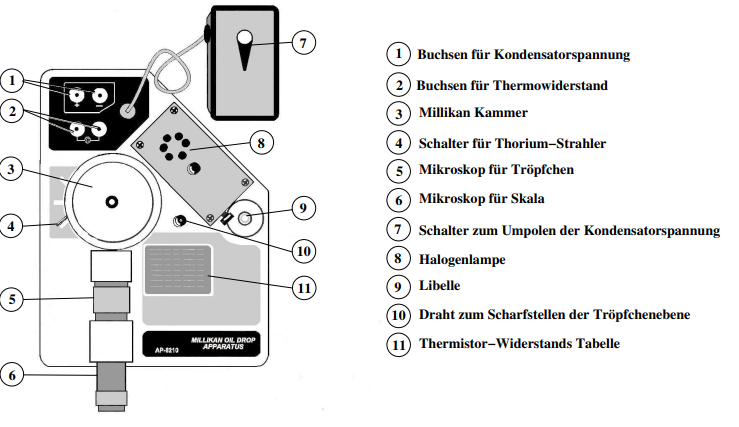
\includegraphics[width = \textwidth]{content/Aufbau.PNG}
    \caption{Skizze des Versuchaufbaus zur Untersuchung von Öltröpfchen im Magnetfeld. \cite{v503}}
    \label{fig:aufbau}
\end{figure}

Zunächst wird damit begonnen die Messapparatur waagerecht aufzustellen, damit die Abweichungen dieser Quelle eleminiert werden können. Dann wird Apparatur angeschaltet. Es 
wird eine Spannung an den Kondensator angelegt, welche in einem Bereich von $\qty{175}{\volt}$ und $\qty{225}{\volt}$ liegen sollte. Bevor die Messung beginnt sollte die 
Lufttemperatur im Kondensator bestimmt werden. Nun wird eine kleine Menge Öl in den Kondensator gesprizt. Dabei sollte das Feld abgeschaltet werden. Dies kann über den 
angeschlossenen Schalter geschehen, über welchen auf die Feldlinienrichtung kontrolliert werden kann. Wurde zu viel Öl in den Kondensator gesprizt ist die Beobachtung 
schwieriger. Daher sollte in diesem Fall das Öl abgelassen werden und nach fünf-minütiger Wartezeit erneut Öl eingeführt werden. 

Nun wird überprüft, ob sich geeignete Öltröpfchen im Kondensator befinden. Dafür wird die Bewegung der Öltröpfchen beobachtet. Bewegen sie sich in einer Angebrachten 
Geschwindigkeit war die Injektion erfolgreich und die Messung kann beginnen. Sollte dies nicht der Fall sein, können die Öltröpfchen über den bereits erwähnten 
$\alpha$-Strahler ionisiert werden, damit die Messung beginnen kann. 

Das Magnetfeld wird nun angeschaltet. Dabei wird die Zeit gemessen, in welcher sich der beobachtete Tropfen um eine bestimmt Strecke fortbewegt. Daraus kann eine Geschwindigkeit
berechnet werden. Dann wird das Feld umgepolt und es wird erneut eine Geschwindigkeit über dieselbe Methode gemessen. Diese beiden Geschwindigkeiten wurden in Abschnitt \ref{HIER SOLL MAN THEORIE KAKA HIN BRATAN DIGAAAAAA}
beschrieben. Pro Tröpfchen sollen die Geschwindigkeiten jeweils drei mal gemessen werden. Außerdem muss eine \textit{Ruhegeschwindigkeit} $v_0$ bestimmt werden. Dazu wird ein 
Öltröpfchen in eine gut beobachtbare Position gebracht und das Magnetfeld ausgeschaltet. Dann wird beobachtet, ob sich der Tröpfen bewegt. Falls das geschieht wird auch hier 
eine Geschwindigkeit gemessen. Zu einer eingestellten Spannung des Kondensators soll diese Messung für fünf Tröpfchen erfolgen. Außerdem soll diese Gesamtmessung für fünf 
verschiedene Spannungen erfolgen. Dabei ist zu beachten, dass die Temperatur während der Messung mehrmals notiert werden sollte, falls sich die Temperatur ändert. 